\section{Evolution Process Analysis}
\label{appendix:evolution}

To demonstrate EVOLVE's self-evolution capability, we conduct a longitudinal experiment tracking how the framework's performance evolves as it processes samples sequentially. We use the RJudge Application domain subset (252 samples) with GPT-4o as the backbone and record metrics using a sliding window of size 30. \emph{Cumulative accuracy} is the classification accuracy computed over all samples processed from the beginning up to the current step, reflecting the framework's overall defense capability as knowledge accumulates, other metrics are similar. As shown in \Fref{fig:evolution_process}, EVOLVE exhibits clear self-evolution behavior across four dimensions:

\begin{figure*}[!t]
    \centering
    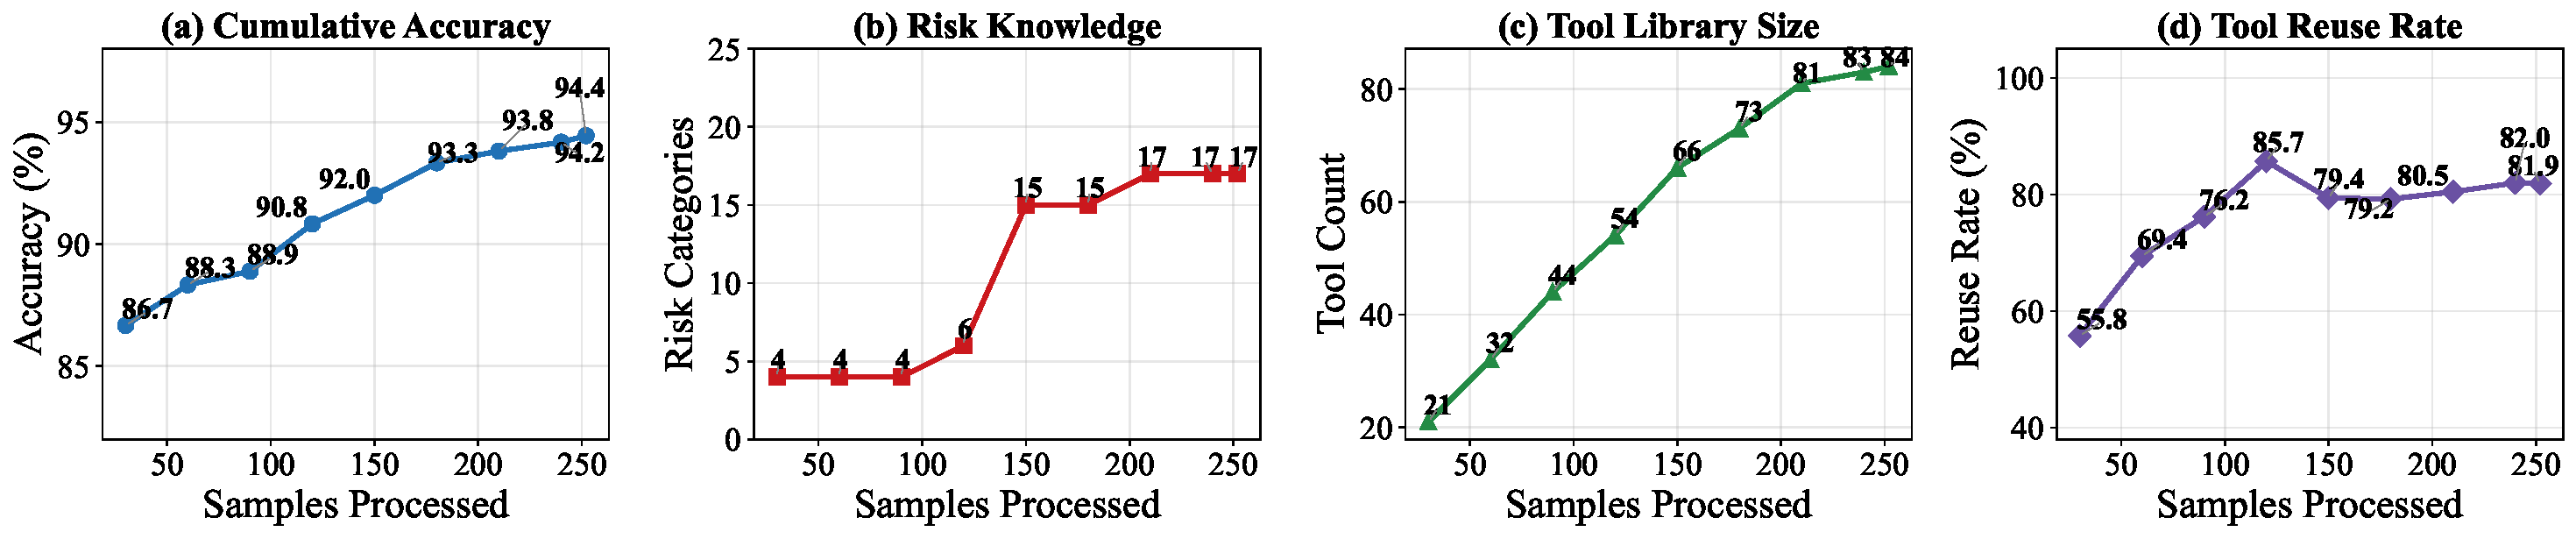
\includegraphics[width=\linewidth]{code/evolution_process.pdf}
    \caption{EVOLVE's evolution process on RJudge (Application domain, GPT-4o). As more samples are processed, the framework progressively improves across all dimensions: (a) cumulative accuracy rises from 86.7\% to 94.4\%; (b) risk knowledge library expands from 4 to 17 categories; (c) tool library grows from 21 to 84 tools; (d) tool reuse rate increases from 55.8\% to 81.9\%.}
    \label{fig:evolution_process}
\end{figure*}

\textbf{Performance improvement.} The cumulative accuracy increases monotonically from 86.7\% (first 30 samples) to 94.4\% (all 252 samples), demonstrating that accumulated security knowledge directly translates into stronger defense capability. The monotonic improvement confirms that newly acquired tools and risk knowledge consistently benefit overall performance rather than introducing regression.

\textbf{Knowledge accumulation.} The risk knowledge library expands from 4 initial categories to 17, with the most significant growth occurring between steps 120--150. This reflects AnalysisAgent's ability to dynamically discover and induct new risk types as it encounters diverse scenarios, without requiring manual rule engineering.

\textbf{Tool library growth.} The guardrail tool library grows steadily from 21 to 84 tools, with each new tool representing externalized security knowledge that can be reused in future interactions. The near-linear growth confirms that EVOLVE continuously generates useful tools rather than saturating early.

\textbf{Reuse rate.} The tool reuse rate rises from 55.8\% to over 80\%, confirming that FusionAgent increasingly leverages existing tools rather than generating redundant ones. This validates the cumulative cultural evolution principle: as the library matures, new risks are more likely to be addressed by adapting existing tools than by creating new ones from scratch.

Together, these trends confirm that EVOLVE is not merely a static defense pipeline but a genuinely self-evolving system whose protective capabilities strengthen through interaction.
